\anhang{Visualisierungen}

\anhangteil{Test Quantum Circuits}\label{q_visual}

Dieses Anhangskapitel, zeigt die Visualisierung aller getetesten \ac{VQC}s.
Die Quelle der entnahme ist in dem Titel der Abbildung angegeben. Die letzte Abbildung zeigt einen neu modifizierten \ac{VQC}, basierend auf bereits vorhandenen Publikationen.
Die Überschriften der Abbildungen, sind im Code verwendeten Variblennamen. Die Publikationen wurden zufällig durchnummeriert.
Aller erstellten Visualisierung wurden im Notebook \code{pa2\_code/visual\_q\_circuits.ipynb} erstellt.



\textbf{Paper 1:}
\begin{figure}[htb]
    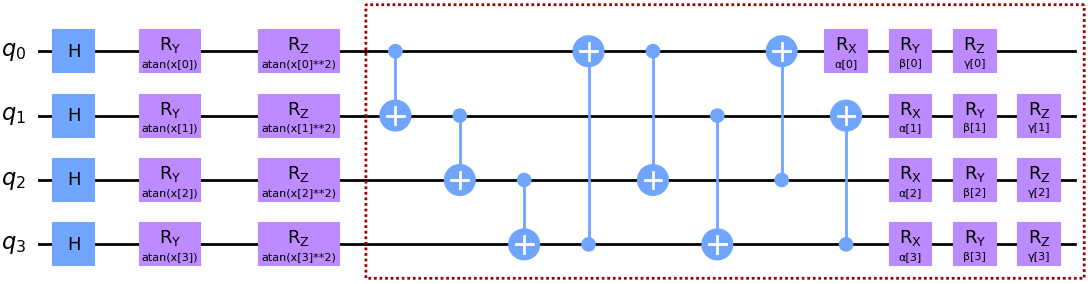
\includegraphics[width=16cm]{lib/graphics/paper_1.png}
    \caption*{Test-\ac{VQC} 1 entnommen aus~\cite{Chen2022}}
    \label{abb:paper1}
\end{figure}

\textbf{Paper 2:}
\begin{figure}[htb]
    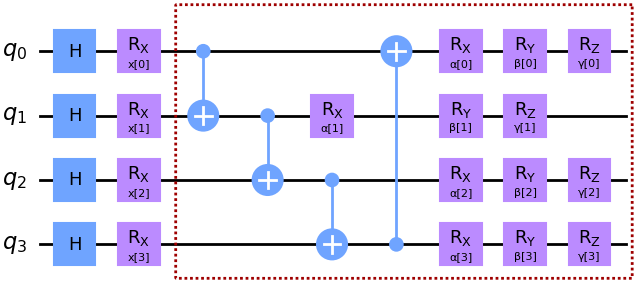
\includegraphics[height=3.9cm]{lib/graphics/paper_2.png}
    \caption*{Test-\ac{VQC} 2 entnommen aus~\cite{Yu2023}}
    \label{abb:paper2}
\end{figure}

\textbf{Paper 3:}
\begin{figure}[htb]
    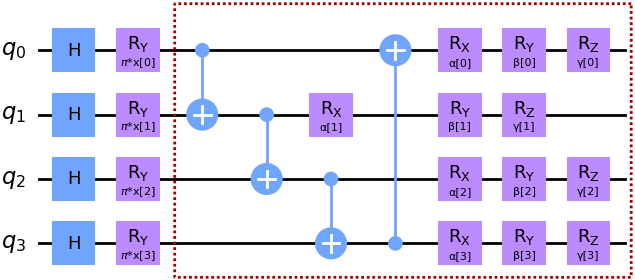
\includegraphics[height=3.9cm]{lib/graphics/paper_3.png}
    \caption*{Test-\ac{VQC} 3 entnommen aus~\cite{Qi2021}}
    \label{abb:paper3}
\end{figure}

\textbf{My\_Own:}
\begin{figure}[htb]
    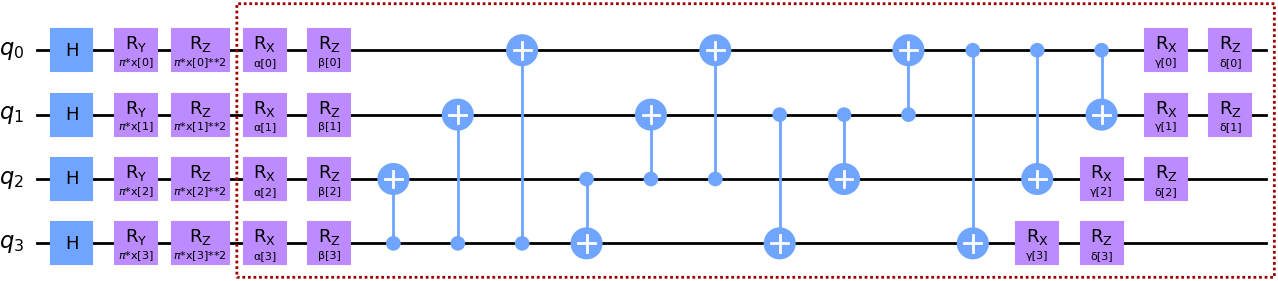
\includegraphics[width=16cm]{lib/graphics/paper_4.png}
    \caption*{Test-\ac{VQC} 4 entnommen aus~\cite{Sim2019} und ~\cite{Chen2022}}
    \label{abb:paper4}
\end{figure}


\anhangteil{Testergebnisse: 4 QLSTM im Vergleich}\label{q_visual}
Lorem Ipsum ist ein einfacher Platzhaltertext für den Druck- und Satzindustrie. Lorem Ipsum hat im Wesentlichen die Norm des Industriestandards seit dem 1500s, als ein unbekannter Drucker eine Hand voll von Typen nahm und sie durcheinander warf, um ein Musterbuch zu machen. Es hat nicht nur fünf Jahrhunderte überlebt, sondern auch den Sprung in die elektronische Schriftbearbeitung, ohne wesentlich zu ändern. Es wurde in den 1960s mit dem Aufkommen von Letraset-Blättern mit Lorem Ipsum-Passagen und mehr kürzlich mit Desktop-Publishing-Software wie Aldus PageMaker einschließlich Versionen von Lorem Ipsum popularisiert.



\newpage